\section{Map}
\label{map}

Auf der Webseite wird die Google-Maps-API benutzt, um einen schnellen Überblick von allen Parks
zu schaffen. Die Google Maps Komponente wurde wie die \nameref{slideshow} Komponente über npm 
heruntergeladen. Der Name der Komponente lautet \textit{google-map-react} und wurde von \textit{istarkov}
und \textit{itsmichaeldiego} erstellt. Auf der Seite wird die Komponente zwei mal benutzt. Der folgende 
Code ist die Map, wo alle Parks eingezeichnet sind.

\begin{code}[htp]
\begin{lstlisting}
    const options = (maps) => {
        return {
            minZoom: 9,
            maxZoom: 20,
            disableDefaultUI: true,
            mapTypeControl: true,
            streetViewControl: true,
            styles: [{ featureType: 'poi', elementType: 'labels', stylers: [{ visibility: 'on' }] }],
        };
  };

    const defaultProps = {
        center: {
            lat: 47.2683,
            lng: 11.3933,
        },
        zoom: 11,
    };
    
    <GoogleMapReact
        options={options}
        bootstrapURLKeys={{ key: Keys }} //API-Key
        defaultCenter={defaultProps.center}
        defaultZoom={defaultProps.zoom}>
        {parks.map(park => (
            <Marker
            lat={park.latitude}
            lng={park.longitude}
            name={park.name}
            color="red"
            link={park.skateparkId}
            />  
        ))}
        {UserLangitude && <Marker
              lat={UserLangitude}
              lng={UserLongitude}
              name="Ihre Position"
              color = "blue"
            />}
      </GoogleMapReact>}
\end{lstlisting}
\caption{React Component - Google map}
\end{code}

In den options, welche als Parameter der Komponente übergeben werden, wird der maximale und minimale Zoom 
definiert, welcher möglich sein soll. Außerdem werden viele Variablen mit dem Wert \textit{true} übergeben, 
welche verschiedene Google-Maps Eigenschaften wie zum Beispiel Street view aktivieren. Der \nameref{apikey}
wird mittels \textit{useFetch} aus einer Textdatei ausgelesen, damit dieser nicht im Quellcode zu 
finden ist. Innerhalb der park Variable, befinden sich die 
Informationen über alle Parks. In der Marker Komponente, wird dann der Breiten- und Längengrad als sowohl auch
der Parkname als Parameter übergeben. Es wird auch die Park ID als Parameter übergeben, um Innerhalb der 
Marker Komponente einen Link zu den Details des jeweiligen Parks zu ermöglichen. Drückt der Benutzer also auf den Marker 
auf eines gewissen Parks, landet er auf dessen Details. Auf der Map wird ebenso ein Marker geladen, dem 
der Längengrad und Breitengrad des Benutzers übergeben wird, um eine bessere Orientierung zu ermöglichen.

\subsection{Marker}

Die Marker selbst sind eine einfache React-Komponente, welche auf die Position des angegeben Längen- und
Breitengrades platziert werden. 

\begin{figure}[H]
    \begin{center}
      \frame{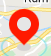
\includegraphics[width=0.1\textwidth]{Website/Marker.png}}
      \caption{Die Startseite}
    \end{center}
\end{figure}

Den Namen welcher dem Markern als Parameter übergeben wird, wird angezeigt, wenn sich die Maus über den 
Marker befindet. Wird dem Marker eine ParkID übergeben, kann dieser dazu benutzt werden die 
View zu einer \nameref{parkDetails}-View zu ändern. Wird dem Marker kein Link Parameter übergeben
passiert beim Drücken des Markers nichts.